\documentclass{training}
\schoollogo{../../resources/intros/UX-03-the-olympics.jpg}
\setlang{french}
\newcommand{\uxfond}{../../resources/fond/UX-03-the-olympics.png}
% Filigrane PAR MODULE : \uxfond (PNG A4 dilue 30 %). Cadre noir vectoriel commun.
% Proportions original 744 px : marge 20/744, trait 1/744. Exterieur BLANC.
% Cadre via eso-pic +\put (coordonnees absolues) — pas de remember picture (decalage).
\usepackage{eso-pic}

\providecommand{\uxfond}{../../resources/fond/norme_fond_paliers_30.png}

\newlength{\uxmargin}
\newlength{\uxthick}
\newlength{\uxinnerw}
\newlength{\uxinnerh}
\setlength{\uxmargin}{0.02688\paperwidth}% 20/744
\setlength{\uxthick}{0.001344\paperwidth}% 1/744
\setlength{\uxinnerw}{\dimexpr\paperwidth-2\uxmargin-2\uxthick\relax}
\setlength{\uxinnerh}{\dimexpr\paperheight-2\uxmargin-2\uxthick\relax}

% Contenu strictement a l'interieur du trait (+ jour confortable).
\geometry{%
  includeheadfoot,
  left=22mm,
  right=22mm,
  top=20mm,
  bottom=18mm,
  headheight=30pt,
  headsep=5mm,
  footskip=12mm%
}

\AddToShipoutPictureBG{%
  \AtPageLowerLeft{%
    % Fond blanc page entiere
    \put(0,0){\color{white}\rule{\paperwidth}{\paperheight}}%
    % Filigrane module a l'interieur du cadre
    \put(\LenToUnit{\dimexpr\uxmargin+\uxthick\relax},\LenToUnit{\dimexpr\uxmargin+\uxthick\relax}){%
      \includegraphics[width=\uxinnerw,height=\uxinnerh]{\uxfond}}%
    % Cadre noir : bas, haut, gauche, droite
    \put(\LenToUnit{\uxmargin},\LenToUnit{\uxmargin}){%
      \color{black}\rule{\dimexpr\paperwidth-2\uxmargin\relax}{\uxthick}}%
    \put(\LenToUnit{\uxmargin},\LenToUnit{\dimexpr\paperheight-\uxmargin-\uxthick\relax}){%
      \color{black}\rule{\dimexpr\paperwidth-2\uxmargin\relax}{\uxthick}}%
    \put(\LenToUnit{\uxmargin},\LenToUnit{\uxmargin}){%
      \color{black}\rule{\uxthick}{\dimexpr\paperheight-2\uxmargin\relax}}%
    \put(\LenToUnit{\dimexpr\paperwidth-\uxmargin-\uxthick\relax},\LenToUnit{\uxmargin}){%
      \color{black}\rule{\uxthick}{\dimexpr\paperheight-2\uxmargin\relax}}%
  }%
}

\makeatletter
\fancyhf{}
\fancyheadoffset{0pt}
\renewcommand{\headrulewidth}{0pt}
\lhead{\parbox[t]{0.56\textwidth}{\RaggedRight\footnotesize\sloppy\@title}}
\rhead{\parbox[t]{0.36\textwidth}{\RaggedLeft\footnotesize\sloppy\@subtitle}}
\cfoot{\thepage}
% Coupures : underscore et slash dans les noms de fichiers / consignes
\DeclareRobustCommand{\_}{\textunderscore\allowbreak}
\makeatother

% Evite les depassements de longues lignes (Github, Name_FirstName_...)
\sloppy
\emergencystretch=3em
\hbadness=10000

% Sommaire type 42 : chapitres seulement
\setcounter{tocdepth}{0}
\renewcommand{\cftchappresnum}{}
\renewcommand{\cftchapaftersnum}{}
\setlength{\cftchapnumwidth}{2.0em}
\setlength{\cftbeforechapskip}{0.35em}
\cftsetindents{chapter}{0em}{2.0em}


\begin{document}

\title{Les Jeux olympiques}
\subtitle{Piscine UX/UI --- UX}
\member{Piscine UX/UI}{https://github.com/01-edu/UX-UI}
\summary{Idéation, parcours, prototype, animation, et un test.}
\version{1.0}
\prerequisite{Le module précédent de cette piscine, ou aucun si c'est le premier.}
\maketitle

\newpage
\tableofcontents
\newpage


\chapter{Instructions}

L'avant-propos n'est pas un exercice. Il ne sera pas noté. Les exercices commencent au chapitre suivant, du contrat le plus simple au plus dur. Un exercice plus tardif n'est pas pris en compte si un plus tôt ne tient pas.

On ne regarde que ce qui est dans le répertoire de rendu de l'exercice. N'ajoutez pas un fichier que l'exercice ne nomme pas. Le nom d'un livrable suit le motif imprimé dans l'exercice : \texttt{Name\_FirstName\_DeliverableName\_Date\_VersionNumber}.

Le geste ne vous est pas donné. Les exemples d'un exercice portent parfois une contrainte que la phrase ne répète pas. Lisez-les. Vos autres références sont le manuel de l'outil choisi, la personne assise à côté, et les liens imprimés dans l'exercice.

L'ordre est celui de la quête. Sauter une étape parce qu'un écran plus tard semble plus intéressant produit un écran que personne ne sait expliquer.

\subsection*{Des images}

La marque en couverture est l'image de ce module. Les paliers pâles derrière le texte sont le fond de page. Ni l'un ni l'autre n'est un indice.

\subsection*{Des machines qui écrivent}

Vous pouvez vous servir d'un outil pour vérifier un mot, comme d'un dictionnaire. Vous ne pouvez pas remplacer un entretien, un test ou un fichier par un texte généré et le signer. Si vous ne pouvez pas montrer la personne, l'écran ou la ligne que vous avancez, l'exercice n'est pas fait.


\chapter{Avant-propos}

En 1972, Otl Aicher a réduit des Jeux à des pictogrammes qu'un visiteur lit sans langue commune. Mexico 1968, avec Lance Wyman, avait déjà montré qu'une identité peut être un système plutôt qu'une mascotte. Regarder les images est permis. Les exercices demandent d'idéer, pas de décalquer ces signes.

\begin{center}
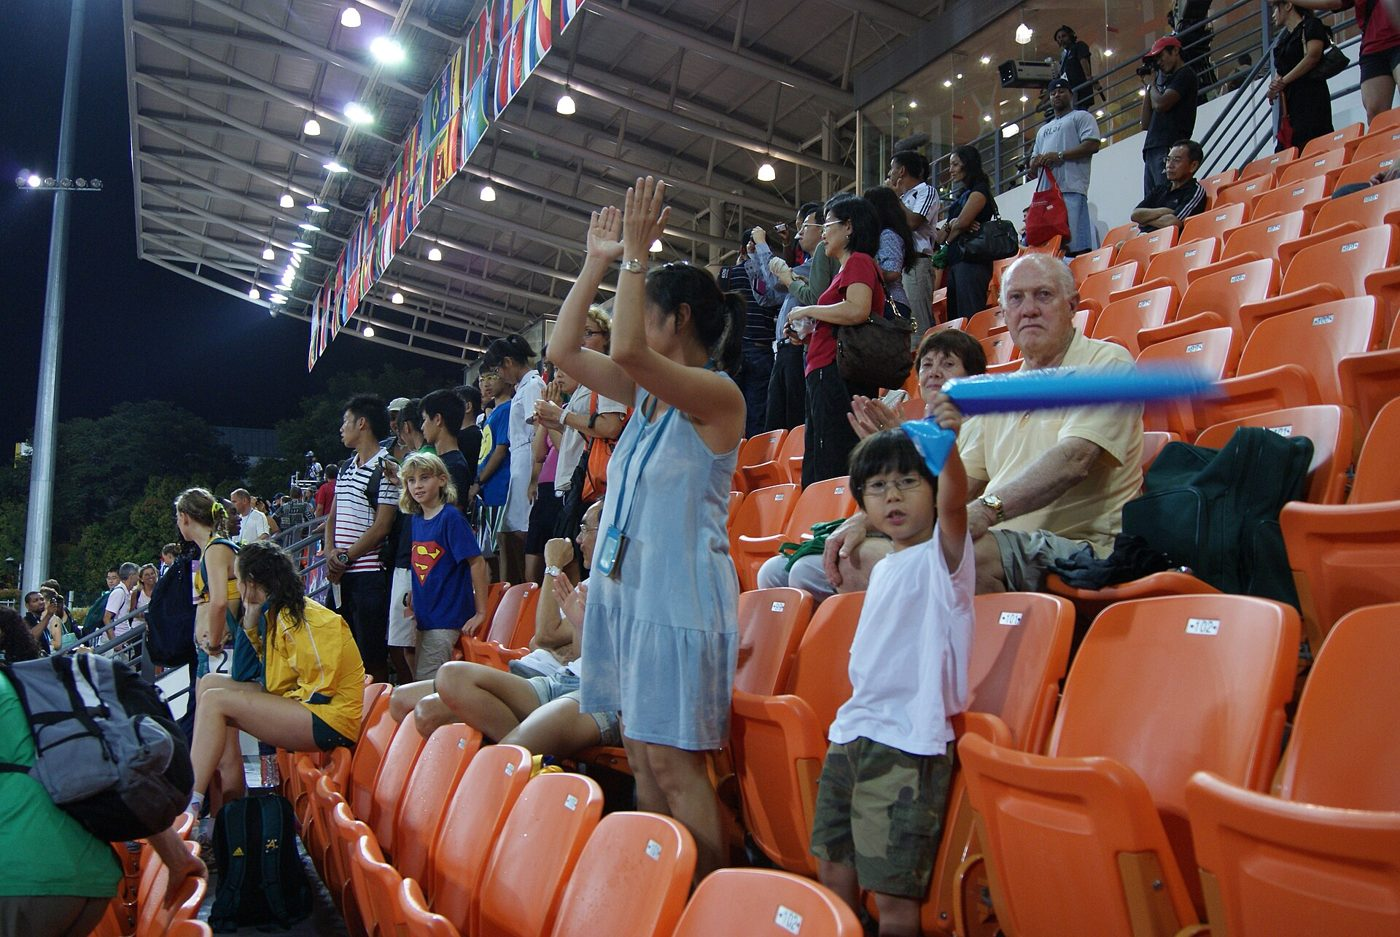
\includegraphics[width=0.78\textwidth,height=0.32\textheight,keepaspectratio]{../../resources/intros/UX-03-the-olympics.jpg}\\[0.4em]
{\footnotesize Image : Jacklee, CC BY-SA 4.0}
\end{center}

À regarder. Les vidéos sont un contexte. Elles ne sont pas le livrable.
\begin{itemize}
\item UX - Introduction \& Quest n°1, 01Edu \url{https://www.youtube.com/watch?v=UbE6WMeuvQg&list=PLHyAJ_GrRtf-RAtfngbRrFh1XDTnyXFDe}
\end{itemize}

\chapter{Exercice 00 : UX IV - Ex 1 - Idéation}
\exnumber{00}
\extitle{UX IV - Ex 1 - Idéation}
\exfiles{ex00/archive zip, nomme Name\_FirstName\_DeliverableName\_Date\_VersionNumber}
\exauthorize{Those named in the exercise}
\makeheaderfiles

\textbf{Contexte :}

The Olympics committee calls on you to get fresh ideas for the next Olympic Games.

You'll team up by groups of 3 and focus each on one problem statement.

You'll get guidelines and suggestions to run ideation workshops, and bring your ideas to life with three different prototypes, that you will animate and test.

\textbf{Instructions :}

Soyons créatifs !

Organize and run an ideation workshop with 4 - 8 participants to find ideas to solve this problem statement:

\textbf{How might we create a digital sport anyone (including athletes, non-athletes, disabled) could play between now and the next Olympics edition?}

A is leader, B is time-keeper and C focuses on logistics

\textbf{Livrables :}

\begin{itemize}
\item A PDF document with the ideation workshop script
\item Des photos de l'atelier en cours
\item A PDF document that represents the main concept out of the workshop
\item Déposez les documents sur Github, dans un zip nommé « ProjectTitle\_Name\_FirstName », et chaque livrable ainsi : « Name\_FirstName\_DeliverableName\_Date\_VersionNumber ». Exemple : « Doe\_John\_MidFiPrototype\_05242024\_V1 ».
\item Ajoutez un titre dans tous les documents écrits.
\item Soignez l'aspect global des livrables. Ils doivent être clairs, simples et lisibles. Vous pouvez regarder canva.com, sans surcharger le dessin de détails.
\end{itemize}

\textbf{Ressources :}

\begin{itemize}
\item Where good ideas come from \url{https://www.ted.com/talks/steven_johnson_where_good_ideas_come_from}
\item Creative Confidence - Book by Tom Keller \url{https://booksvooks.com/creative-confidence-unleashing-the-creative-potential-within-us-all-pdf.html}
\item Sketching (podcast) \url{https://www.usersknow.com/podcast/2016/10/10/ua1wdsszhx2pemugxc1e0qj0a3l9cs}
\item 13 unusual brainstorming methods that work \url{http://www.huffingtonpost.com/young-entrepreneur-council/13-unusual-brainstorming_b_3880619.html}
\item 3 proven methods to organize a brainstorming session \url{https://uxdesign.cc/brainstorm-79e51f20f313}
\item Effective brainstorming (without feeling lost) \url{https://uxdesign.cc/effective-brainstorming-without-being-lost-b68750bbfac5?sk=5d5a332f7e3f2a43364c031b01b13229}
\item The myth of brainstorming \url{https://uxdesign.cc/the-myth-of-brainstorming-8517e02facc0?sk=995d601cbf988d574e86dd71364cb92f}
\item Ideation method: Worst possible idea \url{https://www.interaction-design.org/literature/article/learn-how-to-use-the-best-ideation-methods-worst-possible-idea}
\item Up to you to find more!
\end{itemize}


\chapter{Exercice 01 : UX IV - Ex 2 - Idéation}
\exnumber{01}
\extitle{UX IV - Ex 2 - Idéation}
\exfiles{ex01/archive zip, nomme Name\_FirstName\_DeliverableName\_Date\_VersionNumber}
\exauthorize{Ceux nommés dans l'exercice}
\makeheaderfiles

\textbf{Instructions :}

Soyons créatifs !

Organisez et animez un atelier d'idéation avec 4 à 8 participants pour trouver des idées qui résolvent cet énoncé de problème :

\textbf{Comment pourrions-nous fournir, via notre plateforme, des informations pertinentes et à la demande sur l'impact environnemental et social des Jeux olympiques ?}

B est leader, C est time-keeper et A se concentre sur la logistique.

Attention à ne pas utiliser la même technique d'idéation que dans l'Ex 1 !

\textbf{Livrables :}

\begin{itemize}
\item Un document PDF avec le script de l'atelier d'idéation
\item Des photos de l'atelier en cours
\item Un document PDF qui représente le concept principal issu de l'atelier
\item Déposez les documents sur Github, dans un zip nommé « ProjectTitle\_Name\_FirstName », et chaque livrable ainsi : « Name\_FirstName\_DeliverableName\_Date\_VersionNumber ». Exemple : « Doe\_John\_MidFiPrototype\_05242024\_V1 ».
\item Ajoutez un titre dans tous les documents écrits.
\item Soignez l'aspect global des livrables. Ils doivent être clairs, simples et lisibles. Vous pouvez regarder canva.com, sans surcharger le dessin de détails.
\end{itemize}

\textbf{Ressources :}

\begin{itemize}
\item D'où viennent les bonnes idées \url{https://www.ted.com/talks/steven_johnson_where_good_ideas_come_from}
\item Creative Confidence - Livre de Tom Keller \url{https://booksvooks.com/creative-confidence-unleashing-the-creative-potential-within-us-all-pdf.html}
\item Sketching (podcast) \url{https://www.usersknow.com/podcast/2016/10/10/ua1wdsszhx2pemugxc1e0qj0a3l9cs}
\item 13 méthodes de brainstorming inhabituelles qui fonctionnent \url{http://www.huffingtonpost.com/young-entrepreneur-council/13-unusual-brainstorming_b_3880619.html}
\item 3 méthodes éprouvées pour organiser une session de brainstorming \url{https://uxdesign.cc/brainstorm-79e51f20f313}
\item Brainstorming efficace (sans se sentir perdu) \url{https://uxdesign.cc/effective-brainstorming-without-being-lost-b68750bbfac5?sk=5d5a332f7e3f2a43364c031b01b13229}
\item Le mythe du brainstorming \url{https://uxdesign.cc/the-myth-of-brainstorming-8517e02facc0?sk=995d601cbf988d574e86dd71364cb92f}
\item Méthode d'idéation : la pire idée possible \url{https://www.interaction-design.org/literature/article/learn-how-to-use-the-best-ideation-methods-worst-possible-idea}
\item À vous d'en trouver plus !
\end{itemize}


\chapter{Exercice 02 : UX IV - Ex 3 - Idéation}
\exnumber{02}
\extitle{UX IV - Ex 3 - Idéation}
\exfiles{ex02/archive zip, nomme Name\_FirstName\_DeliverableName\_Date\_VersionNumber}
\exauthorize{Ceux nommés dans l'exercice}
\makeheaderfiles

\textbf{Instructions :}

Soyons créatifs !

Organisez et animez un atelier d'idéation avec 4 à 8 participants pour trouver des idées qui résolvent cet énoncé de problème :

\textbf{Comment pourrions-nous aider les fans de sport à organiser des Jeux olympiques locaux entre 2 éditions internationales ?}

C est leader, A est time-keeper et B se concentre sur la logistique.

Attention à ne pas utiliser la même technique d'idéation que dans l'ex 2 !

\textbf{Livrables :}

\begin{itemize}
\item Un document PDF avec le script de l'atelier d'idéation
\item Des photos de l'atelier en cours
\item Un document PDF qui représente le concept principal issu de l'atelier
\item Déposez les documents sur Github, dans un zip nommé « ProjectTitle\_Name\_FirstName », et chaque livrable ainsi : « Name\_FirstName\_DeliverableName\_Date\_VersionNumber ». Exemple : « Doe\_John\_MidFiPrototype\_05242024\_V1 ».
\item Ajoutez un titre dans tous les documents écrits.
\item Soignez l'aspect global des livrables. Ils doivent être clairs, simples et lisibles. Vous pouvez regarder canva.com, sans surcharger le dessin de détails.
\end{itemize}

\textbf{Ressources :}

\begin{itemize}
\item D'où viennent les bonnes idées \url{https://www.ted.com/talks/steven_johnson_where_good_ideas_come_from}
\item Creative Confidence - Livre de Tom Keller \url{https://booksvooks.com/creative-confidence-unleashing-the-creative-potential-within-us-all-pdf.html}
\item Sketching (podcast) \url{https://www.usersknow.com/podcast/2016/10/10/ua1wdsszhx2pemugxc1e0qj0a3l9cs}
\item 13 méthodes de brainstorming inhabituelles qui fonctionnent \url{http://www.huffingtonpost.com/young-entrepreneur-council/13-unusual-brainstorming_b_3880619.html}
\item 3 méthodes éprouvées pour organiser une session de brainstorming \url{https://uxdesign.cc/brainstorm-79e51f20f313}
\item Brainstorming efficace (sans se sentir perdu) \url{https://uxdesign.cc/effective-brainstorming-without-being-lost-b68750bbfac5?sk=5d5a332f7e3f2a43364c031b01b13229}
\item Le mythe du brainstorming \url{https://uxdesign.cc/the-myth-of-brainstorming-8517e02facc0?sk=995d601cbf988d574e86dd71364cb92f}
\item Méthode d'idéation : la pire idée possible \url{https://www.interaction-design.org/literature/article/learn-how-to-use-the-best-ideation-methods-worst-possible-idea}
\item À vous d'en trouver plus !
\end{itemize}


\chapter{Exercice 03 : UX IV - Ex 4 - Parcours utilisateur}
\exnumber{03}
\extitle{UX IV - Ex 4 - Parcours utilisateur}
\exfiles{ex03/archive zip, nomme Name\_FirstName\_DeliverableName\_Date\_VersionNumber}
\exauthorize{Those named in the exercise}
\makeheaderfiles

\textbf{Instructions :}

Based on the main concept out of the workshop you led, design the user flow a user has to follow to access the main service.

Cet exercice se fait seul.

\textbf{Livrables :}

\begin{itemize}
\item A comprehensive user flow on a board (digital or pictures of a physical one)
\item Déposez les documents sur Github, dans un zip nommé « ProjectTitle\_Name\_FirstName », et chaque livrable ainsi : « Name\_FirstName\_DeliverableName\_Date\_VersionNumber ». Exemple : « Doe\_John\_MidFiPrototype\_05242024\_V1 ».
\item Ajoutez un titre dans tous les documents écrits.
\item Soignez l'aspect global des livrables. Ils doivent être clairs, simples et lisibles. Vous pouvez regarder canva.com, sans surcharger le dessin de détails.
\end{itemize}

\textbf{Ressources :}

\begin{itemize}
\item User flow glossary \url{https://www.productplan.com/glossary/user-flow/}
\item Site flows vs User Flows \url{https://uxmovement.com/wireframes/site-flows-vs-user-flows-when-to-use-which/}
\item How to make a User Flow diagram \url{https://www.lucidchart.com/blog/how-to-make-a-user-flow-diagram}
\end{itemize}


\chapter{Exercice 04 : UX IV - Ex 5 - Prototypage}
\exnumber{04}
\extitle{UX IV - Ex 5 - Prototypage}
\exfiles{ex04/fichier Figma, nomme Name\_FirstName\_DeliverableName\_Date\_VersionNumber}
\exauthorize{Ceux nommés dans l'exercice}
\makeheaderfiles

\textbf{Instructions :}

Donnez une autre dimension à votre user flow et transformez votre user flow en prototype papier (12 écrans max).

D'abord, dessinez des prototypes basse fidélité sur papier. Un écran principal = 1 frame mobile.

Ensuite, dessinez vos écrans mid-fidelity sur Figma avec des formes simples, en noir et blanc.

\textbf{Pistes :} Vocabulaire

\begin{itemize}
\item Basse fidélité : prototypes papier - exemple \url{https://miro.medium.com/max/1400/1*5nUfqqA2gjdAYHagjbHA5w.jpeg}
\item Moyenne fidélité : wireframes, noir et blanc, seulement les éléments principaux, sur un outil de prototype - exemple \url{https://miro.medium.com/max/1400/1*eGSfaxwYbxUFomYbyO6GWw.png}
\item Haute fidélité : wireframes avec couleur, styles, détails graphiques et micro-interactions - exemple \url{https://miro.medium.com/max/1400/1*Xn0HSKAvhr4TZzC9lN5udw.gif}
\end{itemize}

\textbf{Livrables :}

\begin{itemize}
\item Photo d'un prototype papier
\item Un fichier Figma avec les wireframes (moyenne fidélité)
\item Déposez les documents sur Github, dans un zip nommé « ProjectTitle\_Name\_FirstName », et chaque livrable ainsi : « Name\_FirstName\_DeliverableName\_Date\_VersionNumber ». Exemple : « Doe\_John\_MidFiPrototype\_05242024\_V1 ».
\item Ajoutez un titre dans tous les documents écrits.
\item Soignez l'aspect global des livrables. Ils doivent être clairs, simples et lisibles. Vous pouvez regarder canva.com, sans surcharger le dessin de détails.
\end{itemize}

\textbf{Ressources :}

\begin{itemize}
\item Exemple : Prototypage papier - Le guide pratique pour débutants \url{https://www.uxpin.com/studio/blog/paper-prototyping-the-practical-beginners-guide/}
\item Exemple : Application Wellness \url{https://medium.com/@ebtaskin/story-of-my-very-first-ux-ui-design-project-at-ironhack-bootcamp-955addeb760e}
\item Template Mobile Android \url{https://i.pinimg.com/originals/43/8e/de/438ede24264eb9552b635d34142eac29.png}
\item Template iPhone \url{https://www.cssauthor.com/wp-content/uploads/2014/01/iPhone-5S-Template-PSD.jpg}
\item Figma
\end{itemize}

\textbf{Citations :}

\begin{itemize}
\item « Si vous n'êtes pas gêné par la première version de votre produit, vous l'avez lancé trop tard » Reid Hoffman | LinkedIn
\item Pour prototyper votre solution, vous aurez besoin d'un changement temporaire de philosophie : du parfait au juste suffisant, de la qualité à long terme à la simulation temporaire.
\item Le prototype sert à répondre à des questions, donc restez concentré. Vous avez juste besoin d'une façade réaliste à laquelle les clients peuvent réagir.
\end{itemize}


\chapter{Exercice 05 : UX IV - Ex 6 - Animation}
\exnumber{05}
\extitle{UX IV - Ex 6 - Animation}
\exfiles{ex05/fichier Figma, nomme Name\_FirstName\_DeliverableName\_Date\_VersionNumber}
\exauthorize{Those named in the exercise}
\makeheaderfiles

\textbf{Instructions :}

Animate your wireframes on Figma.

Think about multistate!!

Cet exercice se fait seul.

\textbf{Livrable :}

\begin{itemize}
\item An animated Mid-Fi prototype on Figma
\item Déposez le fichier Figma sur Github, nommé ainsi : « Name\_FirstName\_DeliverableName\_Date\_VersionNumber ». Exemple : « Doe\_John\_MidFiPrototype\_05242024\_V1 ».
\item Ajoutez un titre dans le fichier.
\item Soignez l'aspect global du fichier. Il doit être clair, simple et lisible. Vous pouvez regarder canva.com, sans surcharger le dessin de détails.
\end{itemize}

\textbf{Ressources :}

\begin{itemize}
\item Efficiently Manage Your Designs - How Mockplus State Page Helps To View \& Manage Multiple State \url{https://help.mockplus.com/p/372}
\end{itemize}


\chapter{Exercice 06 : UX IV - Ex 7 - Test}
\exnumber{06}
\extitle{UX IV - Ex 7 - Test}
\exfiles{ex06/archive zip, nomme Name\_FirstName\_DeliverableName\_Date\_VersionNumber}
\exauthorize{Those named in the exercise}
\makeheaderfiles

\textbf{Instructions :}

Test your wireframe prototype with 5 different people and write down the 5 main iterations that need to be made on the next version.

Cet exercice se fait seul.

\textbf{Livrables :}

\begin{itemize}
\item A PDF document with the usability test script
\item Des photos des tests en cours
\item A PDF docuemnt with a report on what you learnt and a list of the 5 main iterations that you'd like to do on the next version
\item Déposez les documents sur Github, dans un zip nommé « ProjectTitle\_Name\_FirstName », et chaque livrable ainsi : « Name\_FirstName\_DeliverableName\_Date\_VersionNumber ». Exemple : « Doe\_John\_MidFiPrototype\_05242024\_V1 ».
\item Ajoutez un titre dans tous les documents écrits.
\item Soignez l'aspect global des livrables. Ils doivent être clairs, simples et lisibles. Vous pouvez regarder canva.com, sans surcharger le dessin de détails.
\end{itemize}

\textbf{Ressources :}

\begin{itemize}
\item Running a usability test \url{https://www.usability.gov/how-to-and-tools/methods/running-usability-tests.html}
\item Usability testing: what is it and how to do it? \url{https://uxdesign.cc/usability-testing-what-is-it-how-to-do-it-51356e5de5d}
\item Analyzing usability testing data \url{https://uxdesign.cc/analysing-usability-testing-data-97667ae4999e}
\item The art of guerrilla usability testing \url{http://www.uxbooth.com/articles/the-art-of-guerrilla-usability-testing/}
\item How to write a user testing report that people will actually read \url{https://uxdesign.cc/how-to-write-a-user-testing-report-that-people-will-actually-read-652d15d2f92e}
\end{itemize}

\textbf{Citation :}

Prototypes are created for testing purposes, that's why creating a prototype without running tests on it makes no sense.


\end{document}
